\documentclass[addpoints, 12pt]{exam}
\usepackage[letterpaper,margin=1in]{geometry}
\usepackage{parskip}
\usepackage{graphicx}
\usepackage{isotope}
\usepackage{siunitx}
\usepackage{hyperref}
\usepackage{mhchem}
\usepackage{pst-plot}
\title{Radiometric Dating}
\author{GEOL 189C}
\date{}
\usepackage{libertine}
\usepackage[libertine]{newtxmath}
\begin{document}
\maketitle
\section*{Introduction}
The purpose of this activity is to develop familiarity with the methods used to determine the absolute ages of geologic materials, namely, radiometric dating. Some relevant theoretical and experimental background is included, from which the real tools used by geoscientists are to be derived throughout the course of the activity. 
\subsection*{Absolute Dating}
Absolute dating is the scientific process of answering questions starting with \emph{``when did\ldots''} or \emph{``How long has\ldots''}; in other words, assigning quantitative \emph{ages} to past events. These questions can range in scale from \emph{when did the universe begin?} to \emph{when did this rock form?} to \emph{How long has industrial human society existed?} During this activity, we will develop several tools which are equipped to answer questions like these. In many cases, the question we can answer directly is \emph{when did this rock form?} However, by combining the insights of absolute dating with other tools, we can significantly expand the scope of answerable questions.
\subsection*{Radioactive Decay}
Of the atoms which make up all the matter around us, a considerable number are unstable becuase their nuclei are either too large, too neutron-rich, or too proton rich. These atoms are known as \emph{radionuclides} or described equivalently as \emph{radioactive}. To become more stable, radionuclides spontaneously \emph{decay,} typically by emitting $\alpha$-particles $\left(\isotope[4][2]{He}\right)$, $\beta$-particles (\ce{e-}), or $\gamma$-rays (photons). 

Two key properties of radionuclides allow us to derive a mathematical model which describes their decay.
\begin{enumerate}
	\item There are \emph{many} atoms in any given sample---enough that we can describe them as a continuous amount rather than a discrete number. In other words, each individual atom makes no noticeable difference for the entire sample.
	\item Every copy of a given nuclide---defined by the number of protons and neutrons---is perfectly identical in every way, including the likelihood of decay over a certain interval of time.
	\item In most cases, each parent radioactive nuclide $(P)$ has only one daughter \emph{radiogenic} nuclide $(D)$.
\end{enumerate}
From these assumptions, we can mathematically describe how a sample of radionuclides will decay over time. Since every parent is equally likely to decay, we expect that the amount of decay over a given time interval is proportional to the size of the sample. For example, imagine that from a sample of 100 parent nuclides, 10 decay over 1 year. We would expect that from a sample of \num{1000} parent nuclides, 100 should decay over the same interval. In reality, the actual number of decay events may not exactly match, but the approximation holds for large samples, like the millions or billions of atoms found in a macroscopic sample. 

We generalize by replacing some discrete number of decay events over a dicrete time interval with a new term, the derivative of parent amount $(P)$ with respect to time $t$. This is the left side of our equation. We said this is proportional to the amount $P$ itself, so $P$ must also appear on the right side of the equation. The constant of proportionality is called the decay constant, and the symbol $\lambda$ ``lambda'' is used. Decay constants are experimentally determined and are unique for each given nuclide, based on exactly how unstable it is. The negative sign is added to $\lambda$ because the derivative $dP/dt$ is negative; is time passes, the amount of parent decreases because it is decaying into daughter. Thus we have the governing equation which describes how the amount of radioactive parent changes over time:
\begin{equation}
	\boxed{\frac{dP}{dt}=-\lambda P}\label{decay}
\end{equation}
If we are interested in the amount of daugher nuclide that accumulates over time, we can recognize that it must increase at exactly the same rate that the parent decreases:
\begin{equation}
	\boxed{\frac{dD}{dt}=-\frac{dP}{dt}}\label{parent-daughter}
\end{equation}
As with most governing laws in the natural science, the description of \emph{change over time} is usually the starting point when we look to describe reality in the language of mathematics. Equations like the two above which involve derivatives follow most naturally from our existing theory and relevant observations. However, for the practical purposes of answering specific questions, explaining our observations, and predicting the future, these equations are usually not enough. Why? The essense of the derivative is that it captures are arbitrarily short moment in time, a single snapshot. To be able to recreate the past and predict the future, we would like to derive a tool which allows us to choose any time $t$ and compute the quantity of interest at that moment. For example, we want to be able to select $t=100$ years in the future and calculate the amount of parent which remains and the amount of daughter which has accumulated. 

In the language of functions, we currently have a \emph{differential equation,} an equation which includes differentials (derivatives.) In this case, we start with $dP/dt=f(P)$, meaning ``the derivative of $P$ with respect to $t$ is a function of $P$.'' What we want instead is something of the form $P=f(t)$, meaning ``$P$ is a function of $t$.'' 

To solve this problem we leverage the other fundamental tool of calculus, the integral. Conceptually, we approach the problem this way because the integral continuously adds up each of the infinitesimal moments (captured by the differentials) over some finite interval. We will walk through this procedure step by step, starting with the original decay equation:
\begin{equation}
	\frac{dP}{dt}=-\lambda P\tag{\ref{decay}}
\end{equation}
The first step is to separate the two variables, $P$ and $t$, from one another so that each side of the equation has only a single variable. The mathematical manipulation here is rather subtle, but the end result is that we can ``multiply'' each side by the differential $dt$ so that both $t$ terms are on the right, and divide both sides by $P$ so that both $P$ terms are on the left:
\[\frac{dP}{P}=-\lambda\,dt\]
Note that $\lambda$ is some constant term, so it does not need to be separated. The next step is to realize what our rearranged equation is really saying. The way to interpret left side of the equation is ``some arbitrarily small change in parent amount $dP$, divided by $P$ itself.'' The right side of the equation says ``the negative decay constant, times the arbitrarily small change in time $dt$ (over which that $dP$ occurs).'' It should make sense that these two terms are equal, and that they are conceptually just a different way of expressing the same meaning as equation \ref{decay}. 

The next step is to ``integrate'' each expression, which essentially means to continuously add up all the infinitesimally tiny pieces into a finite length. Again, the rigorous mathematics is very tricky, but this is conceptually the step we're taking. Similarly, it is not worth the time here to dive into the details of why $\int dP/P=\ln(P)$ and $\int dt=t$, but just realize that the integral takes each tiny piece some function and transforms it into another function. 

We also get the term $C$ which is called the constant of integration, and it can take any arbitrary value. We can think of this arbitrary term as an indication that in the process of transformation, we open ourselves up to a whole family of functions which could actually describe the way a system can progress. This is a good sign, becuase it means we can find one member of this family which will best describe the particular details of the question we're interested in. We will see more of what that means later. For now, let's integrate:
\begin{gather*}
	\int\frac{dP}{P}=-\lambda\int dt\\
	\ln P=-\lambda t+C
\end{gather*}
In the next step, we leverage the properties of exponential functions. By raising the constant $e$ to the power of each side of the equation, we can eliminate the natural logarithm.
\begin{gather*}
	e^{\ln P}=e^{-\lambda t+C}\\
	P=e^{-\lambda t+C}
\end{gather*}
Also, we can take a constant term which is added within the exponent and manipulate it in the following way, redefining a slightly different (but still arbitrary) constant $k=e^C$:
\begin{gather*}
	P=e^{-\lambda t+C}\\
	P=e^C\cdot e^{-\lambda t}\\
	P=ke^{-\lambda t}
\end{gather*}
Before moving on, let's take a moment to see what we have done here. With a few manipulations, we have achieved the goal of expressing $P$ as a function of $t$, meaning we can now choose any time and compute exactly the amount of $P$ we should expect! The final step is to deal with this arbitrary constant business and see what it actually means for the problem at hand. Let's define $P_0$ as the amount of parent isotope $P$ we have at time $t=0$. And let's insert these terms into our expression:
\[P_0=ke^{-\lambda (0)}\]
Any number raised to the power of 0 is equal to 1, so we can finally reveal the true identity of $k$:
\[P_0=k\]
That is, $k$ represents the amount of parent we start with whenever we set our timer $t$ to zero. Hopefully, it is now clear why we should expect a whole family of functions which solve our original differential equation \ref{decay}. We need a different function for each initial amount. If we start with a lot of parent, we will expect more of that parent to remain after, say, 10 years, than we would expect for an initial sample with very little parent.
Finally, we can reach the final expression we're looking for, the amount of remaining parent isotope as a function of time:
\begin{equation}
	\boxed{P=P_0\cdot e^{-\lambda t}}
\end{equation}
For those who are familiar with the tools of calculus, you should find the derivative of this expression and confirm that it solves the original differential equation \ref{decay} as we hoped. To build intuition for the characteristics of radioactive systems, it is useful to plot this function for a range of decay constants and check that our expectations, our model, and observable reality are all in agreement.
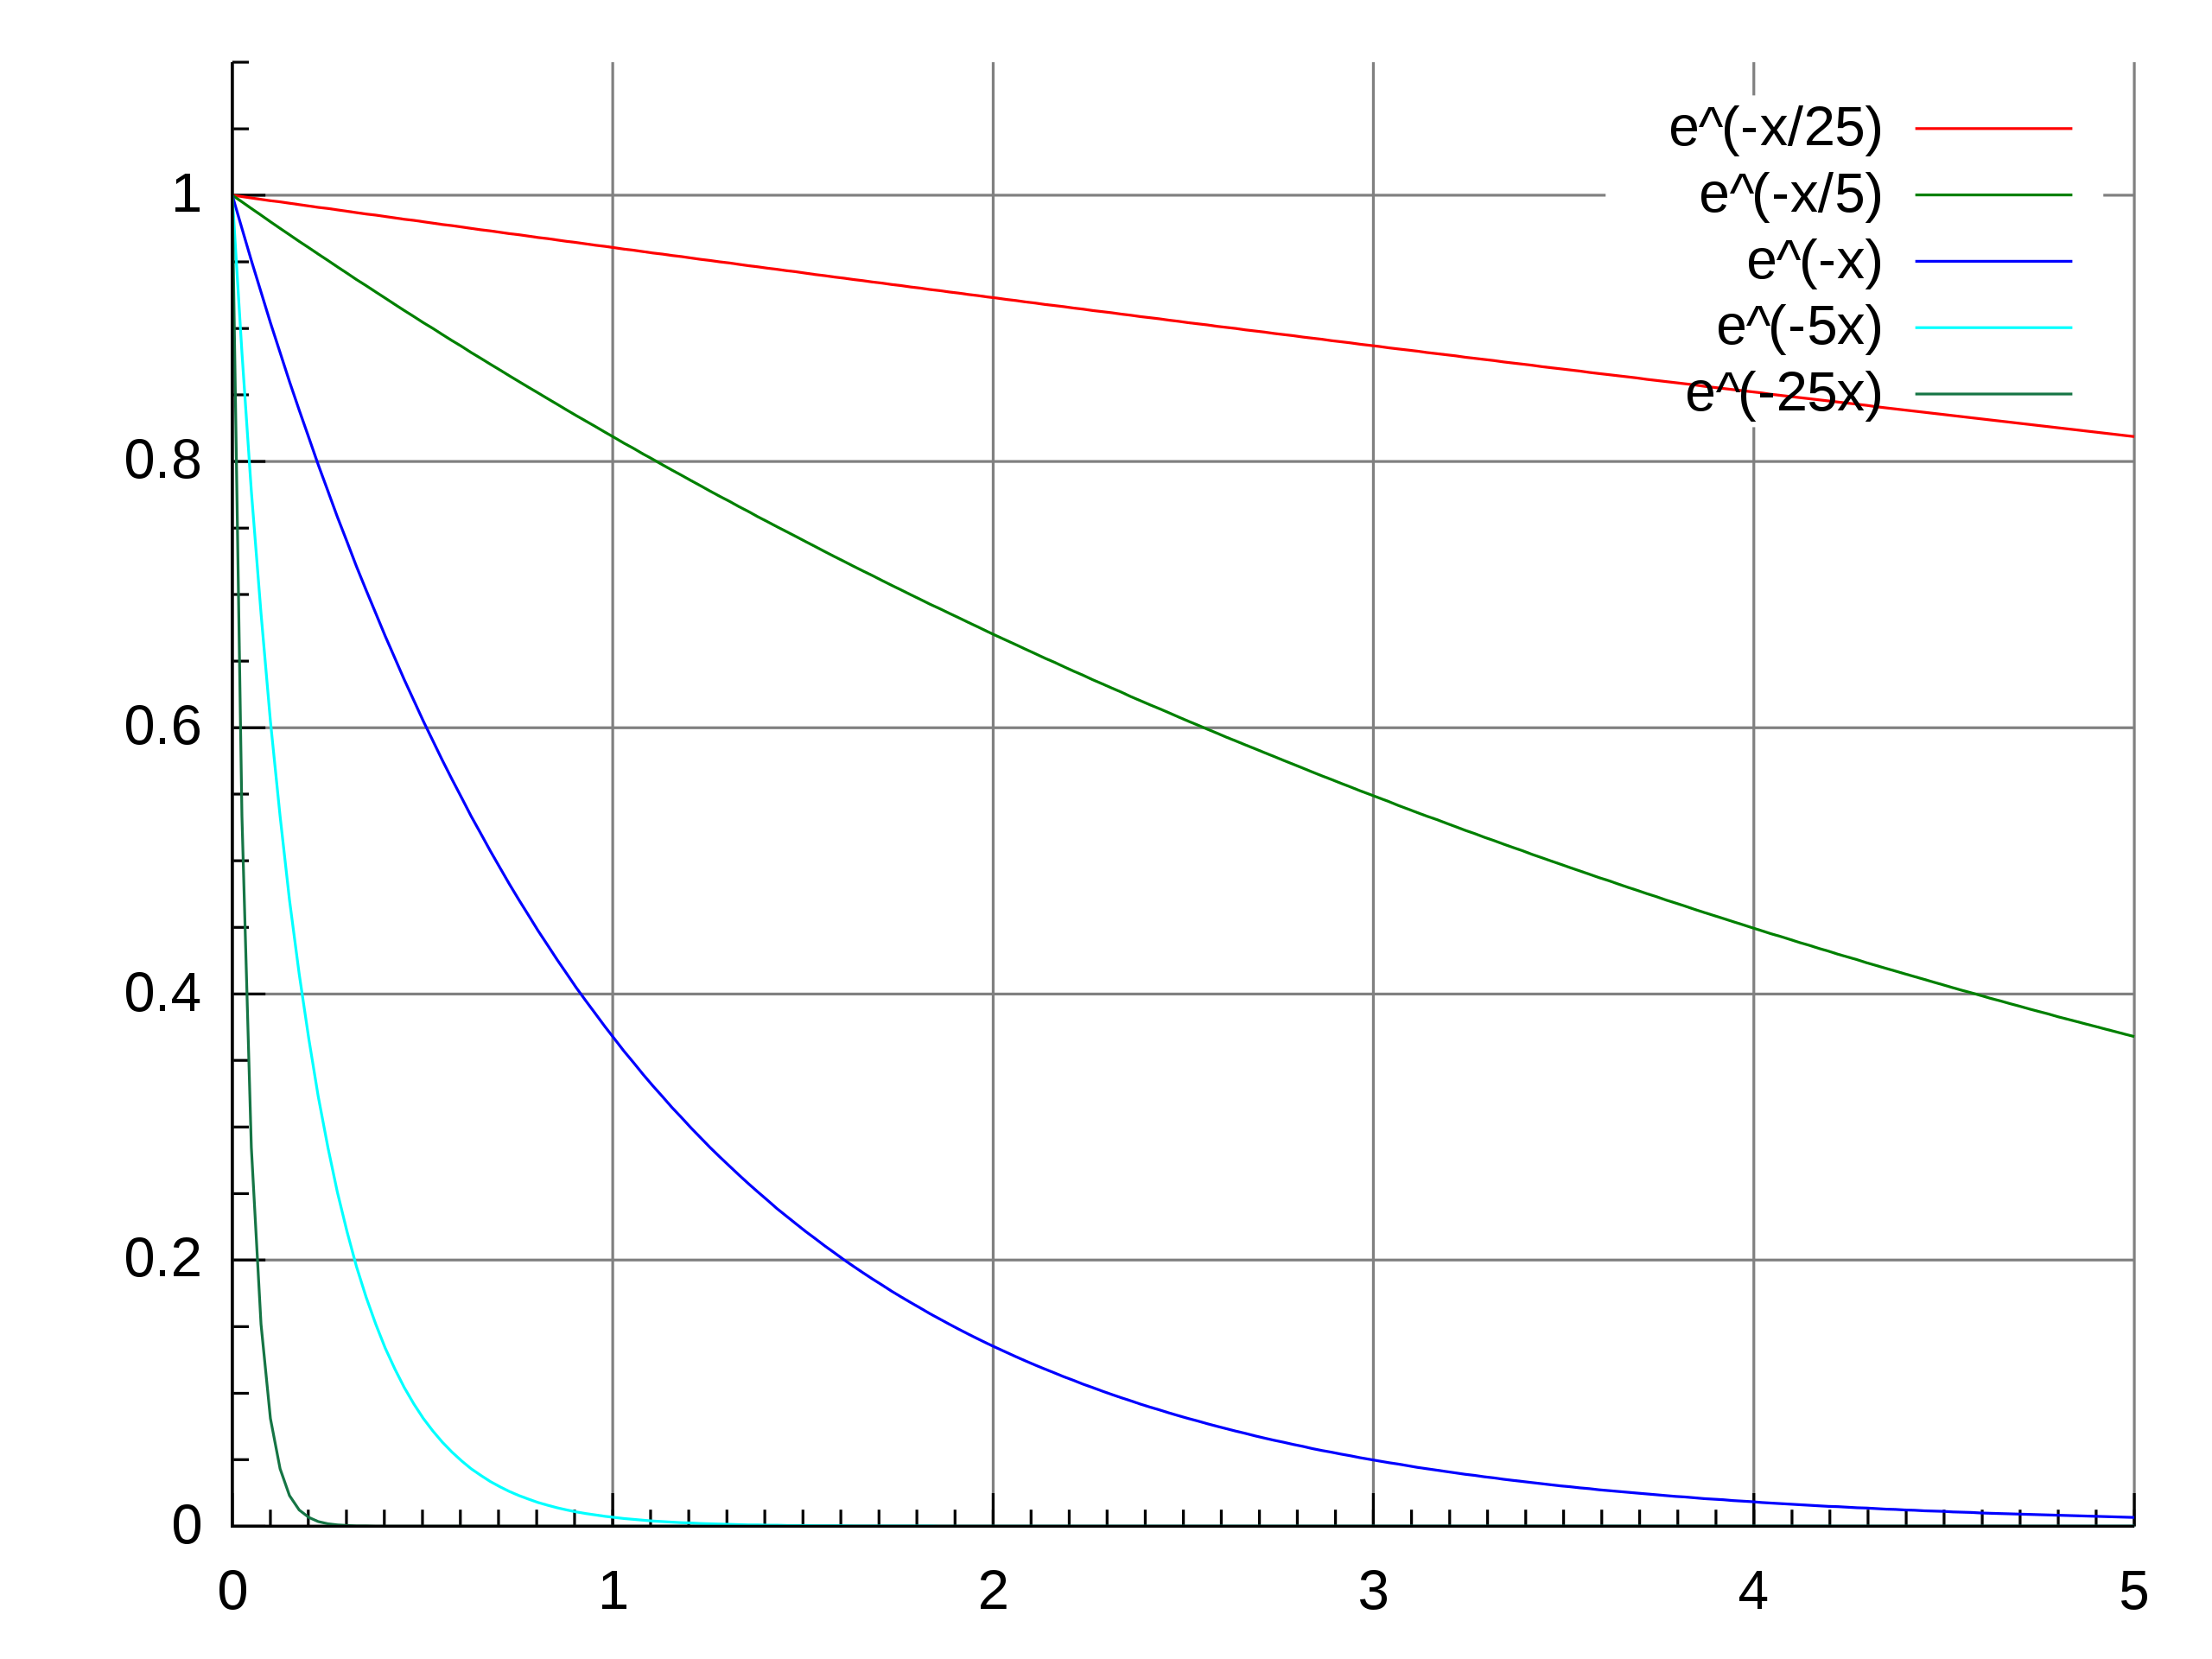
\includegraphics[width=\textwidth]{decay.png}
\subsubsection*{The Half Life}
The decay constant $\lambda$ is in some sense the most fundamental parameter for each radionuclide in that it is necessary for the very formulation of our model in the first place as the constant of proportionality between rate and amount. By carefully examining Equation \ref{decay}, we can see that $\lambda$ must have dimension of inverse time (T$^{-1}$), often expressed in units y$^{-1}$. However, it is somewhat more intuitive to describe a related parameter called the half life $(t_{1/2})$ which is the time it takes for half the parent to decay. Since the rate of radioactive decay is proportional to the amount of parent present, we can show that half life must be independent of amount. We simply solve our equation for $t_{1/2}$ when $P=P_0/2$:
\begin{gather}
	P_0/2=P_0\cdot e^{-\lambda t_{1/2}}\nonumber\\
	1/2=e^{-\lambda t_{1/2}}\nonumber\\
	\ln(1/2)=-\lambda t_{1/2}\nonumber\\
	t_{1/2}=\frac{-\ln(1/2)}{\lambda}\nonumber\\
	\boxed{t_{1/2}=\frac{\ln(2)}{\lambda}}
\end{gather}
With this theoretical background, we are ready to begin building the tools of absolute dating! Futher mathematical constructions will be developed as needed, but these concepts are the common foundation from which the entire field of radiometric dating is built.

In each of the following sections, you will be presented with real or hypothetical data to interpret. In the process, you will build up from first principles the same tools used by professional geoscientists who are interested in quantifying the events and processes of Earth's history. This means you will need to think through the assumptions involved in the geologic context of each sample, the complications which arise when isotope data do not match your expectations, and how to design tools which are best suited to specific problems.

\section{Carbon $\rightarrow$ Nitrogen}
\begin{questions}
\question The half life of \isotope[14]{C} is approximately \qty{5730}{y}. Find the decay constant $\lambda$ for \isotope[14]{C}.
\question \isotope[14]{C} is produced in the upper atmosphere due to reactions between molecular nitrogen and cosmic rays. It is incorporated into carbon-containing gas molecules like \ce{CO2} and \ce{CH4} at a roughly constant rate. The natural abundance of \isotope[14]{C} is roughly 1 part per trillion; the two stable isotopes \isotope[12]{C} and \isotope[13]{C} are far more abundant.
\end{questions}
\section{Rubidium $\rightarrow$ Strontium}
\begin{questions}
\question The half life of \isotope[87]{Rb} is approximately \qty{4.9e10}{y}. Find the decay constant $\lambda$ for \isotope[87]{Rb}.
\end{questions}
\section{Uranium $\rightarrow$ Lead}
\begin{questions}
\question The decay constants of \isotope[235]{U} and \isotope[238]{U} are approximately \qty{9.8485}{y\tothe {-1}} and \qty{1.55125}{y\tothe {-1}}. Find each half life.
\end{questions}
\end{document}
